\section{Model}
\label{sec:model}

\subsection{Overview}
% TODO: Figure of architecture (audio -> encoder -> adapter -> LLM -> text).

\begin{figure}[t]
  \centering
  % 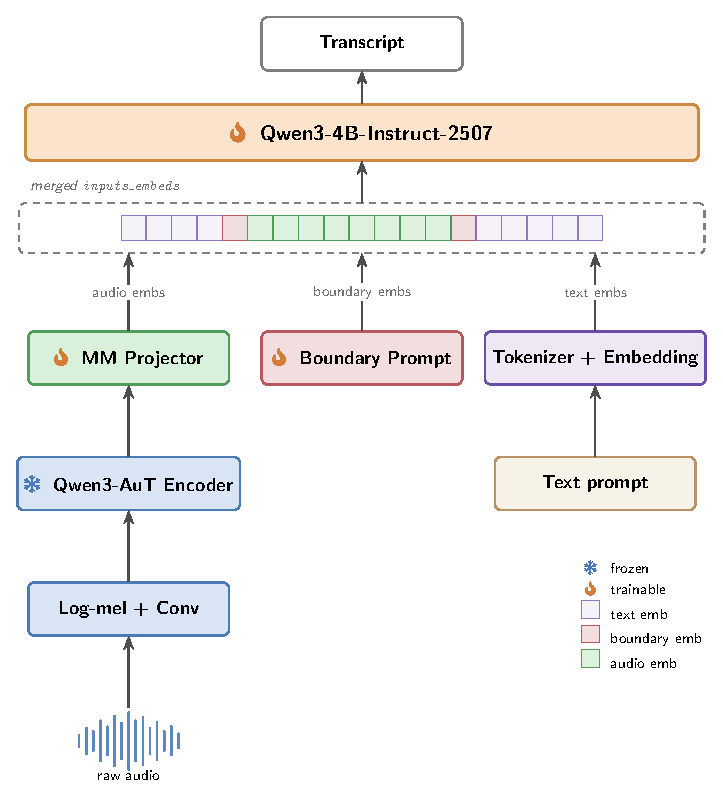
\includegraphics[width=0.85\linewidth]{figures/architecture.pdf}
  \fbox{\rule{0pt}{4cm}\rule{12cm}{0pt}}
  \caption{Overview of LLM-ASR. A speech encoder produces frame-level
    representations that are downsampled by a lightweight adapter and
    consumed as soft prefix tokens by a pre-trained LLM decoder.}
  \label{fig:arch}
\end{figure}

\subsection{Audio Encoder}
% TODO: Whisper-large-v3 encoder / Conformer / your own. Frame rate, dim, params.

\subsection{Adapter}
% TODO: Conv downsampling + Q-Former / linear projection / cross-attention.
% Justify the design and report the parameter count.
The adapter consists of a strided convolutional stack that reduces the
encoder frame rate from 50\,Hz to 12.5\,Hz, followed by a two-layer MLP
that projects to the LLM hidden size.

\subsection{LLM Decoder}
% TODO: Backbone (Qwen2.5 / Llama-3 / your own), size, vocab, context length.

\subsection{Inference}
% TODO: Prompt template, decoding (beam vs. greedy), timestamp / segmentation.

\begin{lstlisting}[caption={Default ASR prompt template.}]
<|system|>
You are a careful speech transcriber. Produce a verbatim transcript
in the language spoken in the audio.
<|audio|>
<|user|>
Transcribe the audio.
<|assistant|>
\end{lstlisting}
